%!TEX root = ../main.tex
\section{Experiments}
\label{sec:experiment}

% \definecolor{shadecolor}{gray}{0.92}

% We evaluate \sys under two different settings including prompting and training. Also, we provide a case study in our technical report~\cite{technical_report} for further understanding of our method.

\begin{table}[t]
  \centering
  \caption{\bf Statistics of datasets.}
  \vspace{-1em}
  \label{tbl:datasets}
  \resizebox{0.93\columnwidth}{!}{
    % 修改列定义：添加了第5列 'c'
    \begin{tabular}{|c||c|c|c|c|}
      \hline
      % 修改表头：添加了 "# Op types" 列，同样使用 multirow 跨两行
      \multirow{2}{*}{\textbf{Dataset}} & \multicolumn{2}{c|}{\textbf{Statistics}} & \multirow{2}{*}{\textbf{Pipeline Length}} & \multirow{2}{*}{\textbf{\# Op Types}} \\ \cline{2-3}
       & \textbf{\# Train} & \textbf{\# Test} & & \\
      \hline \hline
      
      \textbf{Synth-Spider} 
      & 6,788 & 2,008 & 1$\sim$28 & 31 \\ \hline
      
      \textbf{Synth-Bird} 
      & - & 1,150 & 2$\sim$25 & 31 \\ \hline
      
      \textbf{Parrot} ~\cite{ge2025text}
      & 13,965 & 1,365 & 1$\sim$8 & 17 \\
      \hline

      \revise{\textbf{Buildings}~\cite{sharma2023automatic}}
      & \revise{-} & \revise{105} & \revise{-} & \revise{-} \\
      \hline
    \end{tabular}
  }
  \vspace{-1em}
\end{table}

\subsection{Experimental Setup} 
\label{subsec:exp-setup}

\stitle{Datasets.}
As shown in Table~\ref{tbl:datasets}, we evaluate \sys on four datasets, including one public benchmark, two datasets synthesized using our synthesis method, and one real-world dataset. 
% Dataset statistics are summarized in .

(1) \textbf{Parrot}~\cite{ge2025text} is a benchmark for translating natural language into data preparation pipelines.
% However, it does not provide ADP-style task specifications such as target schema descriptions.
To make it suitable for ADP evaluation, we augment each case by generating the task specification from the target tables and operator sequences using an LLM~\cite{doubaoseed}. 
% The resulting dataset contains 15,330 cases with pipeline lengths ranging from 1 to 8.

Note that the public benchmark \textbf{Parrot}~\cite{ge2025text} mainly contains short operator pipelines and limited operator-type coverage. We therefore synthesize two datasets to provide more complex pipelines and broader operator coverage, using our method in Section~\ref{subsec:data_synthesis}. 


(2) \textbf{Synth-Spider} is a dataset synthesized by our method from the Spider NL2SQL benchmark~\cite{spider_dataset}. Using the ADP task synthesis pipeline described in Section~\ref{subsec:data_synthesis}, we convert NL2SQL cases into ADP tasks with executable operator pipelines. 
% The resulting dataset contains 6,788 training cases and 2,008 test cases, with ground-truth pipeline lengths ranging from 1 to 28.

(3) \textbf{Synth-Bird} is another synthesized dataset constructed from the Bird benchmark~\cite{bird_dataset}, which features larger databases and more complex analytical queries. We apply the same synthesis procedure to generate ADP tasks from the Bird validation set.
% , producing 1,150 cases with pipeline lengths ranging from 2 to 25. 
As we use Synth-Bird only for evaluation, this dataset only has test split. 
% Compared to Synth-Spider, this dataset involves longer transformation chains and heavier data processing.

\revise{(4) \textbf{Buildings}~\cite{sharma2023automatic} is a real-world dataset comprising 105 tasks collected from data processing pipelines in the smart building domain across 21 energy companies. It involves messy, real-world data with complex multi-step data preparation operations. It only provides source tables and target table schema descriptions.
% without step-by-step data preparation instructions, reflecting ambiguous data preparation requirements in practice.
}

%\stitle{Datasets.} 
%We evaluate \sys using three datasets, covering both large-scale synthesized scenarios and challenging real-world tasks.
%The statistics of the datasets are shown in Table~\ref{tbl:datasets}.

% \bi
% \item[(1)] \textbf{DP-Spider}~\cite{spider_dataset} is constructed based on the widely-used NL2SQL benchmark Spider~\cite{spider_dataset}. We utilize the Data Synthesis pipeline (Section~\ref{sec:data_synthesis}) to convert the NL2SQL cases into DP cases. It contains 6,788 training samples and 2,008 test samples, with ground truth pipeline lengths ranging from 1 to 28.
% \item[(2)] \textbf{DP-Bird}~\cite{bird_dataset} is derived from the Bird~\cite{bird_dataset} benchmark, known for its large database contents and complex analytical requirements. Compared to DP-Spider, DP-Bird involves longer transformation horizons and more massive data processing. We synthesized cases specifically from the validation set of Bird, constructing 1,150 cases with ground truth pipeline lengths ranging from 2 to 25.
% \item [(3)] \textbf{Parrot}~\cite{ge2025text} is a public dataset originally designed for translating natural language into operator pipeline. It lacks the DP requirements required by NL\nlwhat DP. To address this, we employed Doubao-Seed1.6~\cite{doubaoseed} to generate the DP requirements based on the target tables and operator sequences. Finally, we constructed 15,330 cases with pipeline lengths ranging from 1 to 8. 
% \ei

% \vspace{1mm}
%\noindent
%(1) \textbf{DP-Spider}~\cite{spider_dataset} is constructed based on the widely-used NL2SQL benchmark Spider~\cite{spider_dataset}. We utilize the Data Synthesis pipeline (Section~\ref{subsec:data_synthesis}) to convert the NL2SQL cases into DP cases. It contains 6,788 training samples and 2,008 test samples, with ground truth pipeline lengths ranging from 1 to 28.

% \vspace{1mm}
%\noindent 
%(2) \textbf{DP-Bird}~\cite{bird_dataset} is derived from the Bird~\cite{bird_dataset} benchmark, known for its large database contents and complex analytical requirements. Compared to DP-Spider, DP-Bird involves longer transformation horizons and more massive data processing. We synthesized cases specifically from the validation set of Bird, constructing 1,150 cases with ground truth pipeline lengths ranging from 2 to 25.

% \vspace{1mm}
%\noindent
%(3) \textbf{Parrot}~\cite{ge2025text} is a public dataset originally designed for translating natural language into operator pipeline. It lacks the DP requirements required by NL\nlwhat DP. To address this, we employed Doubao-Seed1.6~\cite{doubaoseed} to generate the DP requirements based on the target tables and operator sequences. Finally, we constructed 15,330 cases with pipeline lengths ranging from 1 to 8. 

\stitle{Evaluation Methodology.}
For comprehensive evaluation, all models are trained only on the \textbf{Synth-Spider} training set and evaluated under two test settings: \emph{in-domain} and \emph{out-of-domain}.

\etitle{(1) In-domain Test.}
We evaluate on the \textbf{Synth-Spider} test set, which is synthesized using the same procedure as the training data.
% but with disjoint queries and databases.

\etitle{(2) Out-of-domain Test.}
% We evaluate on three datasets constructed from different sources and task formats.
\textbf{Synth-Bird} is closer to the training distribution since it is generated by the same synthesis pipeline but from a different benchmark. \textbf{Parrot} is an independent dataset with different task characteristics. \revise{\textbf{Buildings} is a real-world dataset with complex multi-step data preparation.}

%To strictly evaluate the generalization capability of \sys and avoid data leakage, we adopt a \textit{single-source training, multi-target evaluation} protocol. Specifically, we train \sys {exclusively} on the {DP-Spider} training set. The trained model is then evaluated on three distinct test sets.
%DP-Spider Test \textbf{(In-Distribution)}: To assess performance on data with the same distribution as the training set.
%DP-Bird \textbf{(Cross-Domain)}: To evaluate generalization to unseen domains with more complex table schemas, though synthesized via the same pipeline.
%Parrot \textbf{(Out-of-Distribution)}: To evaluate zero-shot transfer capability on a completely independent public benchmark with different data distributions and requirement styles.
%This rigorous setting challenges the model to learn intrinsic DP reasoning logic rather than memorizing dataset-specific patterns.

\stitle{Baselines.} 
We compare \sys with both \emph{prompting baselines} and \emph{training baselines}. Prompting baselines use off-the-shelf LLMs, while training baselines involve parameter updates.
% via supervised or reinforcement learning.
% with various inference strategies


%We compare \sys with two major categories of baselines: \textit{Prompting Baselines} and \textit{Training Baselines}.
% \textit{Prompting Baselines}, which utilize off-the-shelf LLMs with various inference strategies, and \textit{Training Baselines}, which involve parameter updates via supervised or reinforcement learning.

\etitle{(1) Prompting Baselines.} These methods use frozen LLMs with different planning and search strategies to generate pipelines.
%
\begin{itemize}[leftmargin=*]
    \item CodeGen~\cite{li2024towards,sapkota2025vibe} prompts an LLM to iteratively generate and execute data preparation code
    % execute it, observe the output and refine the code 
    until the target table is obtained.
    % from source tables.
    \item {Plan-and-Solve (PaS)}~\cite{wang2024chain} prompts an LLM to produce a plan and then generates an operator pipeline to obtain the target table. 
    % using a two-stage strategy that first produces a high-level plan and then generates a complete operator sequence to obtain the target table.
    \item {ReAct}~\cite{aksitov2023rest} is a linear reasoning agent that iteratively predicts the next operator based on previous execution results.
    \item {MCTS-OP}~\cite{li2025alphasql} applies Monte Carlo Tree Search (MCTS) over individual operators defined in Section~\ref{subsec:operator_space}
    % , using local node expansion and scalar rewards to guide search. We follow the framework of~\cite{li2025alphasql} and keep parameters as default.
    \item {MontePrep}~\cite{ge2025monteprep} applies MCTS over actions such as schema mapping, operator discovery, code synthesis, and refinement instead of individual operators. 
    % We use the released code with default settings.
    % instead of individual operators. We use the authors’ released code with default settings.
    \item {DeepAnalyze}~\cite{zhang2025deepanalyze} is an agentic LLM that generates data processing programs using supervised and reinforcement learning.
    \item {AutoPrep}~\cite{fan2024autoprep} is a multi-agent framework for data preparation. It generates a high-level plan and then produces data preparation programs through specialized agents.
    % Since it does not cover as many operators as our setting, we extend it following its original design.
    \item \revise{{TRAE} and Claude Code (CC) are AI-powered coding agents with agentic coding capabilities. We evaluate them as representative state-of-the-art agentic coding systems\footnote{We use CC v2.1.119 and TRAE from \url{https://github.com/bytedance/trae-agent}.}.}
\end{itemize}

%\noindent


%(1) \textbf{Prompting Baselines}. This category utilizes off-the-shelf LLMs with various inference strategies
% is further divided into three subgroups based on the reasoning paradigm.

% We implement two \textit{Direct Prompting} baselines. These methods rely on the reasoning capability of LLMs without complex iterative frameworks.

%    \underline{{CodeGen}}~\cite{li2024towards,sapkota2025vibe} directly prompts the LLM to output the target data preparation code based on the input tables and target schema.
%    
%    \underline{{Plan-and-Solve (PaS)}}~\cite{wang2024chain} adopts a two-stage strategy where it first analyzes the input tables and NL requirements (Plan) and then generates a complete sequence of operators that will be executed to obtain the target table.

% We compare with three \textit{Agentic Frameworks}. These methods employ iterative interaction loops to refine solutions.
%
%    \underline{{AutoPrep}}~\cite{lai2025auto} is a multi-agent framework focusing on table reconstruction and column transformation. It first generates a high-level DP plan with a Planner agent and then assigns several Programmer agents to implement specific DP programs. Since it does not consider multiple tables and data cleaning operators, we extend its capabilities following its original design.
%    
%    \underline{{ReAct}}~\cite{aksitov2023rest} predicts the next operator from the operator space defined in Section~\ref{subsec:operator_space} based on the execution results of previous steps, representing a standard linear reasoning agent.
    
    % \underline{{CodeGen}}~\cite{sapkota2025vibe} is an iterative framework that interacts with a Python interpreter. It generates code blocks, executes them, and observes outputs to refine the code until the task is completed.

% We compare with two \textit{Search-based Frameworks}. These methods explore the solution space explicitly to find optimal paths.
%
%    \underline{{MCTS-OP}}: This method applies Monte Carlo Tree Search to the operator space defined in Section~\ref{subsec:operator_space}, relying on local node expansion and scalar rewards to navigate the search for DP operators. We follow~\cite{li2025alphasql} to design the MCTS framework and keep all parameters consistent with its public code repository.
%    
%    \underline{{MontePrep}}~\cite{ge2025monteprep}. Different from MCTS-OP, it defines five action types including \texttt{SchemaMapping}, \texttt{OperatorDiscovery}, \texttt{CodeSynthesis}, \texttt{CodeRefinement}, and \texttt{Termination} as atomic search units instead of DP operators. We implement MontePrep with their published code and keep all parameters as default.
%    
%    \underline{{DeepAnalyze}}~\cite{zhang2025deepanalyze} is a code agent model built upon Qwen3-8B. It conduct an SFT+RL training on data science tasks and leverages an CodeGen architecture. It achieves state-of-the-art (SOTA) performance in data analysis and report generation tasks.

\etitle{(2) Training Baselines.} These baselines use the same backbone models as \sys but adopt different training strategies, allowing us to evaluate the effect of our agentic training framework.
\begin{itemize}[leftmargin=*]
    % \item {Imitation Learning (IL)}~\cite{li2025llms} fine-tunes the model on the high-quality reasoning trajectories distilled from strong teacher models (\eg DeepSeek-R1). Unlike standard SFT on (input, output) pairs, this baseline learns the step-by-step reasoning process.
    \item {Imitation Learning (IL)}~\cite{li2025llms} fine-tunes the model on the high-quality trajectories distilled from strong teacher models.
    % (\eg DeepSeek-R1). Unlike standard SFT on (input, output) pairs, this baseline learns the step-by-step reasoning process.
    \item {RL-GRPO}~\cite{shao2024deepseekmath} applies reinforcement learning with Group Relative Policy Optimization using only outcome-level rewards.
    % , without our curriculum and hybrid reward design.
\end{itemize}


\revise{
\stitle{Prompt Design and Tuning for Baseline Methods.} 
Specifically, (1) for methods with public implementations, i.e., MontePrep~\cite{ge2025monteprep}, DeepAnalyze~\cite{zhang2025deepanalyze}, AutoPrep~\cite{fan2024autoprep}, and MCTS-Op~\cite{li2025alphasql}, we use their official codebases and default configurations (e.g., prompt design, parameters, etc.). 
When a method was designed for a different task and could not be directly applied to ADP, we adapted its prompt to the ADP setting and tuned its parameters using the same grid-search procedure adopted by \sys. For example, AutoPrep was designed for TableQA rather than autonomous data preparation, so we replaced its original prompt with an ADP-oriented prompt and tuned it accordingly.
(2) For methods without public implementations, including CodeGen, ReAct, and PaS, we reimplemented them following the descriptions in their papers and applied the same prompt-tuning and parameter-selection procedure used for \sys. Therefore, all methods were evaluated under a comparable tuning method. Complete prompts, hyperparameters, and implementation details are provided in our technical report~\cite{technical_report}.
}




%\noindent
%(2) \textbf{Training Baselines}. These methods train the backbone models for the data preparation task.
%
%    \underline{{SFT}} refers to Standard Supervised Fine-Tuning, where models are trained on the tree-based reasoning trajectories distilled from SOTA LLMs (\eg Claude-4). 
%    
%    \underline{{RL-GRPO}}~\cite{shao2024deepseekmath} refers to Reinforcement Learning with Group Relative Policy Optimization. This baseline optimizes the model directly using outcome rewards.
     % (\eg execution success) to encourage correct final tables without relying solely on ground-truth paths.

\stitle{Evaluation Metrics.}
We evaluate all methods using three metrics.

\etitle{(1) Exact Match Accuracy (Acc.)} measures the percentage of test cases where the produced table $\hat{T}$ matches the ground-truth table $T^*$. We follow the table matching method in~\cite{ge2025text}, which is invariant to row and column permutations but requires exact cell-value equality.

\etitle{(2) Completion Rate (Comp.)} measures the percentage of test cases that produce a final output table. A case is counted as incomplete if execution exceeds the maximum interaction limit, triggers runtime errors, or produces an empty result.

% \etitle{(3) Inference Cost (Cost)} measures the average monetary cost per case. For closed-source LLMs, we compute API cost using official pricing. For open-source models, we measure per-case end-to-end runtime under parallel requests and convert it to cost using the hourly price of the GPU instance. Specifically, the cost of case $i$ is computed as
% $c_i = p_{\text{gpu}} \cdot t_i / 3600$,
% and we report the average over all cases. We use an A800-80G GPU priced at \$0.91/hour ({\url{https://cloud.vast.ai/}).

\etitle{(3) Inference Cost (Cost)} measures the average monetary cost per case. For closed-source LLMs, we use official API pricing. For open-source models, we convert end-to-end runtime to cost using the hourly GPU price:
$c_i = p_{\text{gpu}} t_i / 3600$,
where $t_i$ is the runtime in seconds. We report the average over all cases, using an A800-80G GPU priced at \$0.91/hour.

%\stitle{Evaluation Metrics.} 
%We adopt four metrics for evaluation.

% % \vspace{1mm} \noindent
% \vspace{1mm}
%\noindent
%{(1) {\bf Exact Matching Accuracy (Acc.).}}
%We measure the percentage of test cases where the method produces a target table $\hat{T}$ that exactly matches the ground truth table $T^*$.
%We adopt the table matching protocol from \cite{ge2025text}, which accounts for row/column permutation invariance but strictly checks for cell value equality.

% % \vspace{1mm} \noindent
% \vspace{1mm}
%\noindent
%{(2) {\bf Completion Rate (Comp.).}}
%We calculate the percentage of test cases where the method successfully yields a final output table.
%A failure is recorded if the agent exceeds the maximum interaction turns, raises runtime exceptions or generates empty table.

% % \vspace{1mm} \noindent
% \vspace{1mm}
%\noindent {(3) {\bf Inference Cost.}} We quantify the the economic efficiency of all methods. For methods based on closed-sourced LLMs, we calculate the API cost based on the official pricing policy with the caching mechanism. For methods based on open-source LLMs, we deploy the models on rented GPU servers using vLLM, and measure the per-case end-to-end processing time under parallel client requests. We then convert the time cost into monetary cost using the cloud provider's hourly rental price. Specifically, let $p_{\text{gpu}}$ denote the on-demand price (USD/hour) of the GPU instance, and $t_i$ denote the processing time (seconds) of case $i$ measured under the target concurrency. the inference cost is computed as $c_i = p_{\text{gpu}} \cdot \frac{t_i}{3600}$, and we report the average cost over all cases, \ie $\bar{c} = \frac{1}{N}\sum_{i=1}^{N} c_i$. Specifically, we deploy the model on server with one A800-80G GPU, which is priced by \$0.91 per hour\footnote{\url{https://cloud.vast.ai/}}.


% {(3) {\bf API Cost.}} \fmh{Maybe Inference Cost? \$0.91 per hour per A800 gpu on \url{https://cloud.vast.ai/}} % https://getdeploying.com/gpus/nvidia-a800
% % 或者在AWS上 A100的价格算：%4.10 per hour
% We quantify the economic efficiency by calculating the average API cost for each case.
% The cost estimation is based on the official pricing policy with the {context caching} mechanism.
% % This metric highlights the trade-off between DP performance and financial costs in real-world scenarios.

% \noindent
% {(4) {\bf Latency.}}
% We measure the time efficiency by recording the average consumed time required for open-source models to complete a task.
% To ensure fair comparison, we perform inferences on a single NVIDIA A800 GPU and disable parallel invocation strategies.

\stitle{Backbone LLMs and \sys Variants.}
We implement \sys on both closed-source and open-source LLM backbones.

\etitle{(1) Closed-source backbones.}
We implement \sys with our proposed tree-based agentic reasoning directly on the strongest proprietary models, including GPT-5 (\ie gpt-5-mini-2025-08-07) and Claude-4 (\ie claude-sonnet-4-20250514).

\etitle{(2) Open-source backbones.}
We implement \sys based on open-source LLMs, \ie Qwen2.5~\cite{hui2024qwen2} (with {0.5B}, {1.5B}, {3B}, {7B} and 14B parameters) and Qwen3~\cite{yang2025qwen3} ({0.6B}, {1.7B}, {4B}, {8B} and 14B). 
% For these models, we apply our agentic training procedure and then evaluate them with the same inference framework.

\subsection{Overall Comparison}
\label{expsec:overall_comparison}

\begin{table}[t]
    \centering
    \caption{\bf 
    Comparison of \sys with baselines on open-source LLMs. The best and second-best results are highlighted in \textbf{bold} and \underline{underlined}, respectively.
    % Results on more LLMs (0.5B, 1.5B, 3B, 7B, 14B models of Qwen2.5 and 0.6B, 1.7B, 4B models of Qwen3) can be found in our technique report~\cite{technical_report}.
    }
    \label{tbl:opensource_exp}
    \vspace{-1em}

    % =======================================================
    % Subtable 5: Open-Source & Training - Qwen3-14B
    % =======================================================
    \begin{subtable}[t]{0.9\columnwidth}
        \centering
        \caption{\bf{Results on Qwen3-14B.}}
        \label{subtbl:open_qwen14b}
        \vspace{-0.5em}
        \resizebox{0.99\linewidth}{!}{
        \begin{tabular}{|c||c|c||c|c|c|c|}
            \hline
            \multirow{2}{*}{\textbf{Method}} & \multicolumn{2}{c||}{\textbf{Synth-Spider}} & \multicolumn{2}{c|}{\textbf{Synth-Bird}} & \multicolumn{2}{c|}{\textbf{Parrot}} \\ \cline{2-7}
             & \textbf{Acc.} & \textbf{Comp.} & \textbf{Acc.} & \textbf{Comp.} & \textbf{Acc.} & \textbf{Comp.} \\
            \hline \hline
            \multicolumn{7}{|c|}{\cellcolor{gray!10}\textit{Prompting Baselines}} \\
            % CodeGen & 41.83 & 67.08\% & 27.74 & 48.71\% & 31.52 & 86.16\% \\
            PaS & 7.67 & 20.67\% & 3.09 & 21.86\% & 9.56 & 22.36\% \\
            MCTS-OP & 21.91 & 72.56\% & 7.22 & {78.69\%} & 24.95 & 83.02\% \\
            MontePrep & 9.46 & 19.62\% & 18.63 & 38.15\% & 26.94 & 57.87\% \\
            AutoPrep & 36.75 & 71.61\% & 10.41 & 39.89\% & 28.54 & 74.05\% \\
            CodeGen & 45.47 & 68.18\% & 29.48 & 49.20\% & 30.83 & 81.08\% \\
            ReAct & 40.39 & 69.02\% & 16.04 & 46.56\% & 30.80 & 76.44\% \\
            \hline \hline
            \multicolumn{7}{|c|}{\cellcolor{gray!10}\textit{Training Methods (Only Trained on Synth-Spider)}} \\
            % IL & \underline{59.61} & \underline{88.65\%} & \underline{44.16} & 74.75\% & \underline{34.58} & 
            IL & \underline{61.70} & \underline{85.26\%} & \underline{48.01} & \underline{81.23\%} & \underline{37.95} & \underline{89.39\%} \\
            RL-GRPO & 51.22 & 77.68\% & 32.25 & 67.22\% & 35.06 & 82.9\% \\ \hline
            \begin{tabular}{@{}c@{}}\textbf{\sys}\\ \textbf{(Ours)}\end{tabular} & \textbf{67.18} & \textbf{97.21\%} & \textbf{54.09} & \textbf{92.26\%} & \textbf{40.44} & \textbf{96.41\%} \\
            \hline
        \end{tabular}
        }
    \end{subtable}

    \vspace{0.5em}
    
    % =======================================================
    % Subtable 4: Open-Source & Training - Qwen3-8B
    % =======================================================
    \begin{subtable}[t]{0.9\columnwidth}
        \centering
        \caption{\bf{Results on Qwen3-8B.}}
        \label{subtbl:open_qwen8b}
        \vspace{-0.5em}
        \resizebox{0.99\linewidth}{!}{
        \begin{tabular}{|c||c|c||c|c|c|c|}
            \hline
            \multirow{2}{*}{\textbf{Method}} & \multicolumn{2}{c||}{\textbf{Synth-Spider}} & \multicolumn{2}{c|}{\textbf{Synth-Bird}} & \multicolumn{2}{c|}{\textbf{Parrot}} \\ \cline{2-7}
             & \textbf{Acc.} & \textbf{Comp.} & \textbf{Acc.} & \textbf{Comp.} & \textbf{Acc.} & \textbf{Comp.} \\
            \hline \hline
            \multicolumn{7}{|c|}{\cellcolor{gray!10}\textit{Prompting Baselines}} \\
            % CodeGen & 29.53 & 45.22\% & 19.12 & 32.52\% & 24.25 & 56.27\% \\
            PaS & 4.68 & 7.42\% & 0.65 & 4.33\% & 3.09 & 8.32\% \\
            MCTS-OP & 12.90 & 15.19\% & 0.90 & 73.56\% & 17.33 & 23.71\% \\
            MontePrep & 8.81 & 19.97\% & 13.70 & 21.96\% & 25.95 & 56.08\% \\
            AutoPrep & 26.44 & 50.85\% & 8.52 & 42.28\% & 25.20 & 70.42\% \\
            CodeGen & 6.27 & 12.10\% & 7.47 & 15.69\% & 7.27 & 25.50\% \\
            ReAct & 29.63 & 52.59\% & 10.41 & 46.22\% & 22.11 & 57.97\% \\
            DeepAnalyze & 35.66 & 82.02\% & 1.74 & 62.17\% & 29.01 & 66.67\% \\
            \hline \hline
            \multicolumn{7}{|c|}{\cellcolor{gray!10}\textit{Training Methods (Only Trained on Synth-Spider)}} \\
            % IL & \underline{58.62} & \underline{92.63\%} & \underline{41.63} & \underline{83.98\%} & \underline{33.26} & \underline{91.36\%} \\ % 2025 Version
            IL & \underline{59.65} & \underline{90.54\%} & \underline{43.30} & \underline{80.43\%} & \underline{36.15} & \underline{91.08\%} \\
            RL-GRPO & 47.81 & 76.54\% & 29.95 & 68.69\% & 32.82 & 85.05\% \\ \hline
            \begin{tabular}{@{}c@{}}\textbf{\sys}\\ \textbf{(Ours)}\end{tabular} & \textbf{65.99} & \textbf{97.46\%} & \textbf{53.39} & \textbf{92.78\%} & \textbf{39.93} & \textbf{98.46\%} \\
            \hline
        \end{tabular}
        }
    \end{subtable}
    \vspace{-1em}
\end{table}

% \begin{table}[t]
    \centering
    \caption{\bf Comparison of \sys and baselines on SOTA LLMs. Results on more LLMs (DoubaoSeed1.6-Thinking, DeepSeek-V3.1 and DoubaoSeed1.6-flash) can be found in our technique report ~\cite{technical_report}.}
    \label{tbl:sota_exp}
    \vspace{-1em}

    % =======================================================
    % Subtable 2: SOTA - Claude-4
    % =======================================================
    \begin{subtable}[t]{\columnwidth}
        \centering
        \caption{\bf{Results on SOTA LLMs (Backbone: Claude-4).}}
        \label{subtbl:sota_claude}
        \vspace{-0.15em}
        \resizebox{0.99\linewidth}{!}{
        \begin{tabular}{|c||c|c|c|c|c|c|}
            \hline
            \multirow{2}{*}{\textbf{Method}} & \multicolumn{2}{c|}{\textbf{DP-Spider}} & \multicolumn{2}{c|}{\textbf{DP-Bird}} & \multicolumn{2}{c|}{\textbf{Parrot}} \\ \cline{2-7}
             & \textbf{Acc.} & \textbf{Comp.} & \textbf{Acc.} & \textbf{Comp.} & \textbf{Acc.} & \textbf{Comp.} \\
            \hline \hline
            CodeGen & 59.51 & 86.65\% & 50.55 & 70.27\% & 40.44 & 91.93\% \\ 
            PaS & 46.91 & 79.83\% & 27.59 & 61.55\% & 41.19 & 93.43\% \\
            MCTS-OP & 66.58 & \underline{99.05\%} & 58.91 & \underline{95.32\%} & 41.68 & 98.51\% \\
            MontePrep & 44.27 & 59.46\% & 26.05 & 45.37\% & 41.93 & 69.72\% \\
            AutoPrep & 63.70 & 97.01\% & 46.71 & 91.24\% & 40.79 & \underline{99.15\%} \\
            CodeGen & 62.05 & 82.82\% & 57.62 & 73.85\% & 41.14 & 92.83\% \\
            ReAct & \underline{69.92} & 96.86\% & \underline{59.91} & 89.09\% & \underline{42.88} & 96.12\% \\
            \hline
            \begin{tabular}{@{}c@{}}\textbf{\sys}\\ \textbf{\textsc{-P} (Ours)}\end{tabular} & \textbf{73.46} & \textbf{99.85\%} & \textbf{67.43} & \textbf{97.91\%} & \textbf{46.07} & \textbf{99.70\%} \\
            \hline
        \end{tabular}
        }
    \end{subtable}

    \vspace{0.5em}

    % =======================================================
    % Subtable 1: SOTA - GPT-5
    % =======================================================
    \begin{subtable}[t]{\columnwidth}
        \centering
        \caption{\bf{Results on SOTA LLMs (Backbone: GPT-5).}}
        \label{subtbl:sota_gpt}
        \vspace{-0.15em}
        \resizebox{0.99\linewidth}{!}{
        \begin{tabular}{|c||c|c|c|c|c|c|}
            \hline
            \multirow{2}{*}{\textbf{Method}} & \multicolumn{2}{c|}{\textbf{DP-Spider}} & \multicolumn{2}{c|}{\textbf{DP-Bird}} & \multicolumn{2}{c|}{\textbf{Parrot}} \\ \cline{2-7}
             & \textbf{Acc.} & \textbf{Comp.} & \textbf{Acc.} & \textbf{Comp.} & \textbf{Acc.} & \textbf{Comp.} \\
            \hline \hline
            CodeGen & 62.90 & 92.73\% & 55.88 & 83.96\% & 38.40 & 93.33\% \\
            PaS & 52.29 & 85.26\% & 36.65 & 73.85\% & 39.39 & 95.32\% \\
            MCTS-OP & 61.55 & \underline{97.41\%} & 47.71 & \textbf{95.02\%} & 33.72 & \textbf{99.20\%} \\
            MontePrep & 41.09 & 65.14\% & 27.14 & 51.00\% & \textbf{42.98} & 85.21\% \\
            AutoPrep & 51.54 & 82.87\% & 45.42 & 79.63\% & 38.25 & 85.96\% \\
            CodeGen & 64.39 & 92.38\% & 56.82 & 89.89\% & 40.29 & 95.72\% \\
            ReAct & \underline{67.03} & 97.31\% & \underline{57.37} & \underline{93.38\%} & 40.19 & {96.36\%} \\ % re-run the exp
            \hline
            \begin{tabular}{@{}c@{}}\textbf{\sys}\\ \textbf{\textsc{-P} (Ours)}\end{tabular} & \textbf{71.76} & \textbf{98.21\%} & \textbf{60.46} & 92.53\% & \underline{41.33} & \underline{97.26\%} \\
            \hline
        \end{tabular}
        }
    \end{subtable}

    \vspace{0.5em}

    % =======================================================
    % Subtable 3: SOTA - DeepSeek-R1
    % =======================================================
    \begin{subtable}[t]{\columnwidth}
        \centering
        \caption{\bf{Results on SOTA LLMs (Backbone: DeepSeek-R1).}}
        \label{subtbl:sota_dsr1}
        \vspace{-0.15em}
        \resizebox{0.99\linewidth}{!}{
        \begin{tabular}{|c||c|c|c|c|c|c|}
            \hline
            \multirow{2}{*}{\textbf{Method}} & \multicolumn{2}{c|}{\textbf{DP-Spider}} & \multicolumn{2}{c|}{\textbf{DP-Bird}} & \multicolumn{2}{c|}{\textbf{Parrot}} \\ \cline{2-7}
             & \textbf{Acc.} & \textbf{Comp.} & \textbf{Acc.} & \textbf{Comp.} & \textbf{Acc.} & \textbf{Comp.} \\
            \hline \hline
            CodeGen & 56.23 & 86.11\% & 52.09 & 76.99\% & 36.06 & 93.53\% \\
            PaS & 44.92 & 72.66\% & 34.41 & 51.34\% & 35.86 & 89.69\% \\
            MCTS-OP & \underline{62.10} & \textbf{96.07\%} & 50.85 & \textbf{95.77\%} & 33.02 & 95.32\% \\
            MontePrep & 33.52 & 53.54\% & 17.63 & 33.22\% & \textbf{42.58} & 82.77\% \\
            AutoPrep & 54.53 & 84.61\% & 40.09 & 89.49\% & 33.17 & 96.96\% \\
            CodeGen & 59.71 & 78.09\% & 45.27 & 65.49\% & 35.91 & 88.30\% \\
            ReAct & 59.11 & 85.91\% & \underline{59.31} & \underline{89.64\%} & 38.84 & \underline{97.21\%} \\ 
            \hline
            % \textbf{\sys-P (Ours)} & \textbf{65.23} & \underline{93.92\%} & \textbf{60.16} & 88.65\% & \underline{39.64} & \textbf{98.26\%} \\
            \begin{tabular}{@{}c@{}}\textbf{\sys}\\ \textbf{\textsc{-P} (Ours)}\end{tabular} & \textbf{65.23} & \underline{93.92\%} & \textbf{60.16} & 88.65\% & \underline{39.64} & \textbf{98.26\%} \\
            \hline
        \end{tabular}
        }
    \end{subtable}

    
\end{table}


% \begin{figure}[t]
    \centering
    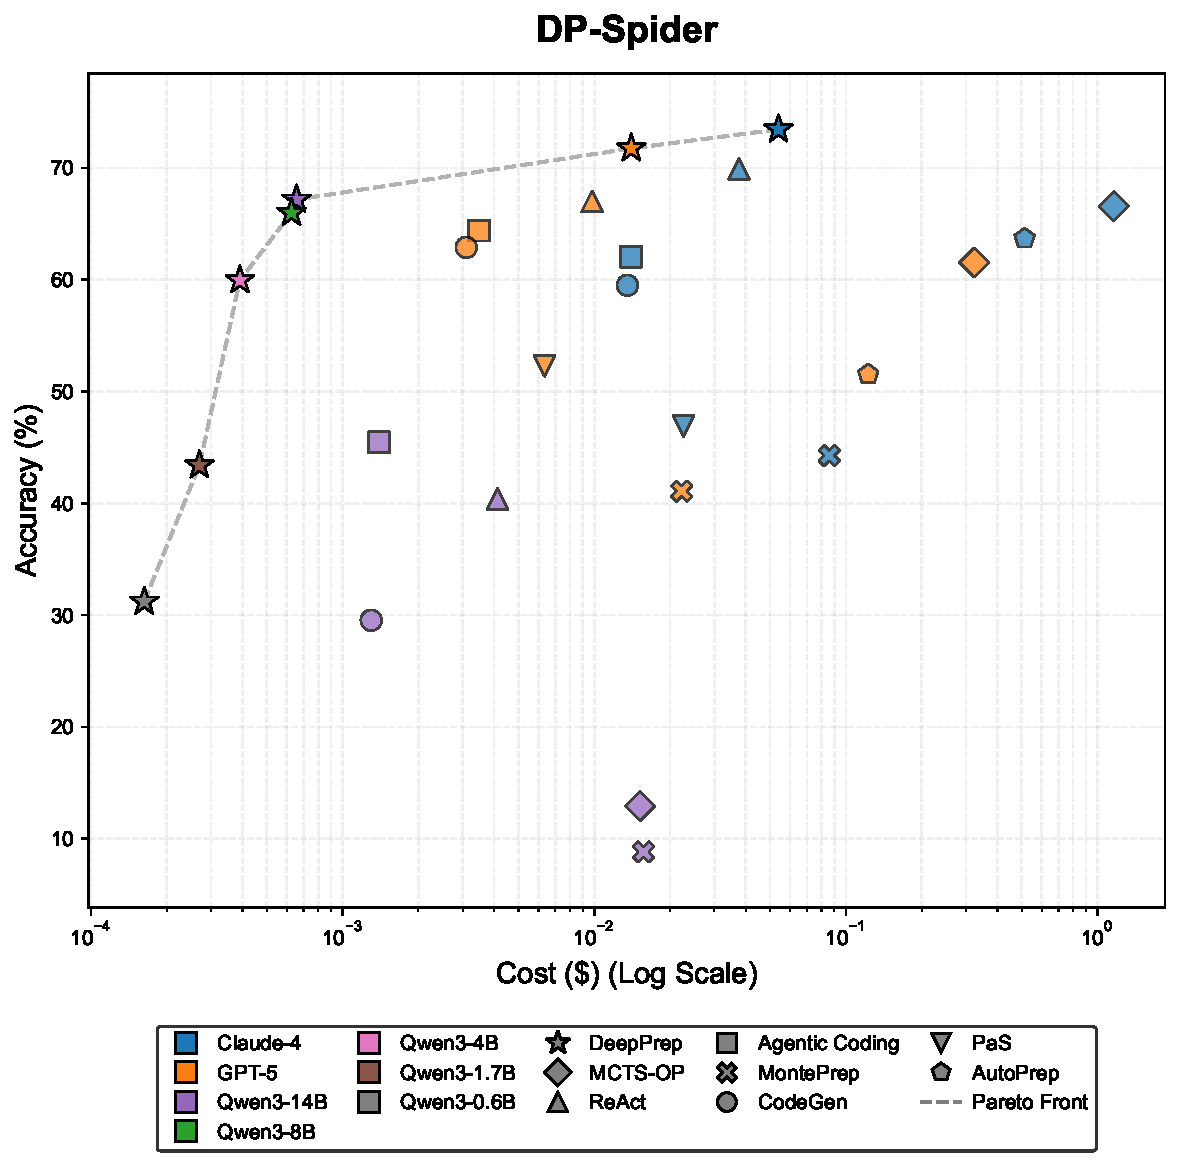
\includegraphics[width=0.99\columnwidth]{plots/plot/pareto_front_spider.pdf}
    \vspace{-1em} 
    \caption{Pareto Front on DP-Spider.}
    \label{fig:pareto_front_spider}
    % \vspace{-1em}
\end{figure}
% \begin{figure}[t]
    \centering
    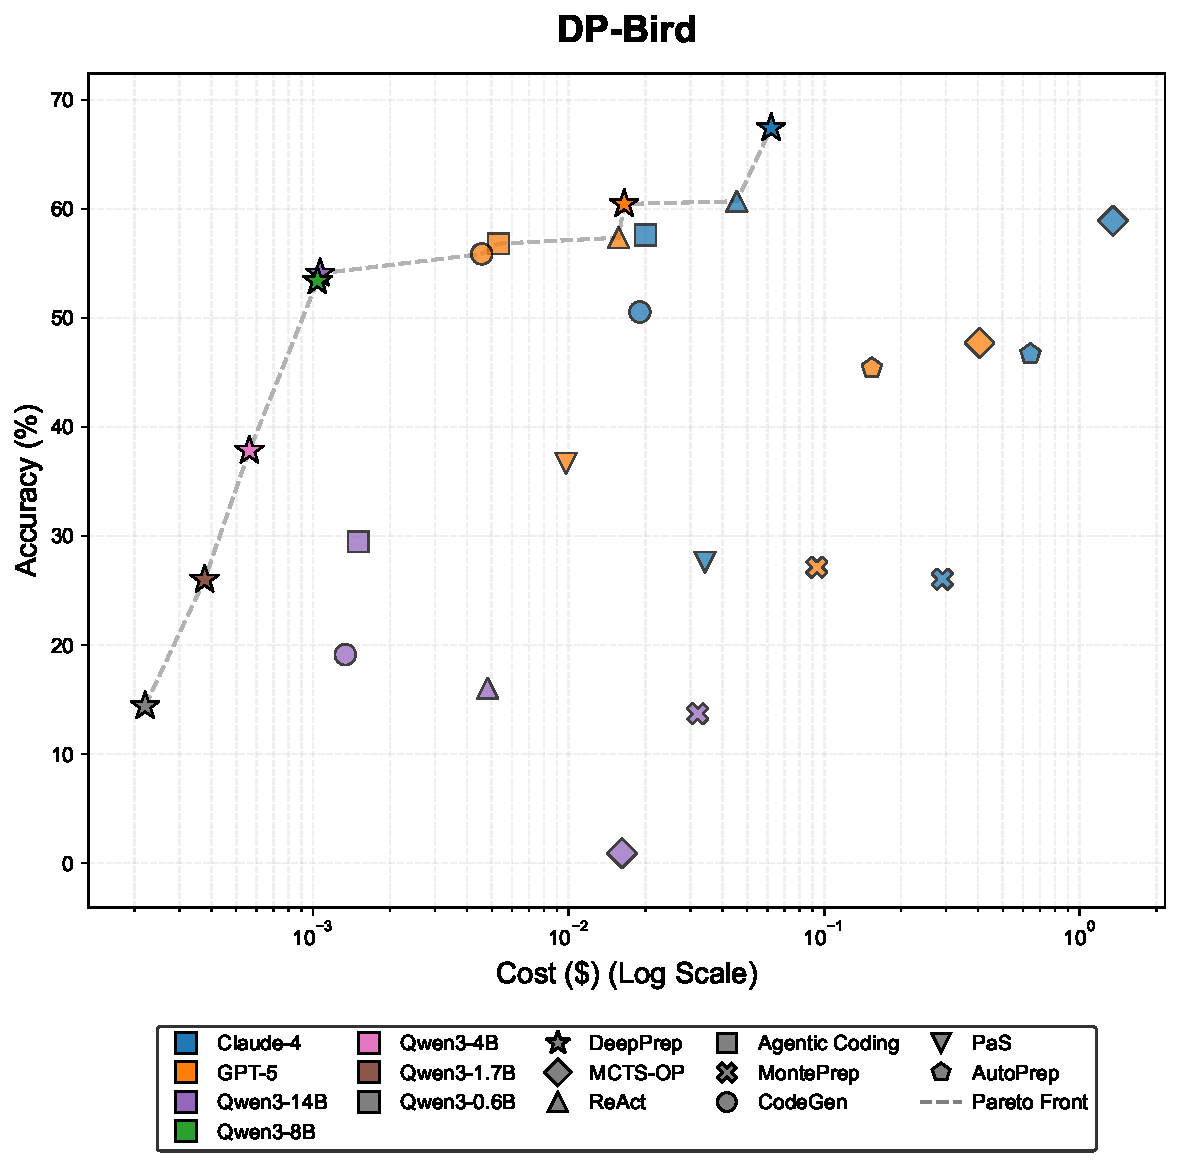
\includegraphics[width=0.99\columnwidth]{plots/plot/pareto_front_bird.pdf}
    \vspace{-1em} 
    \caption{Pareto Front on DP-Bird.}
    \label{fig:pareto_front_bird}
    % \vspace{-1em}
\end{figure}
% \begin{figure}[t]
    \centering
    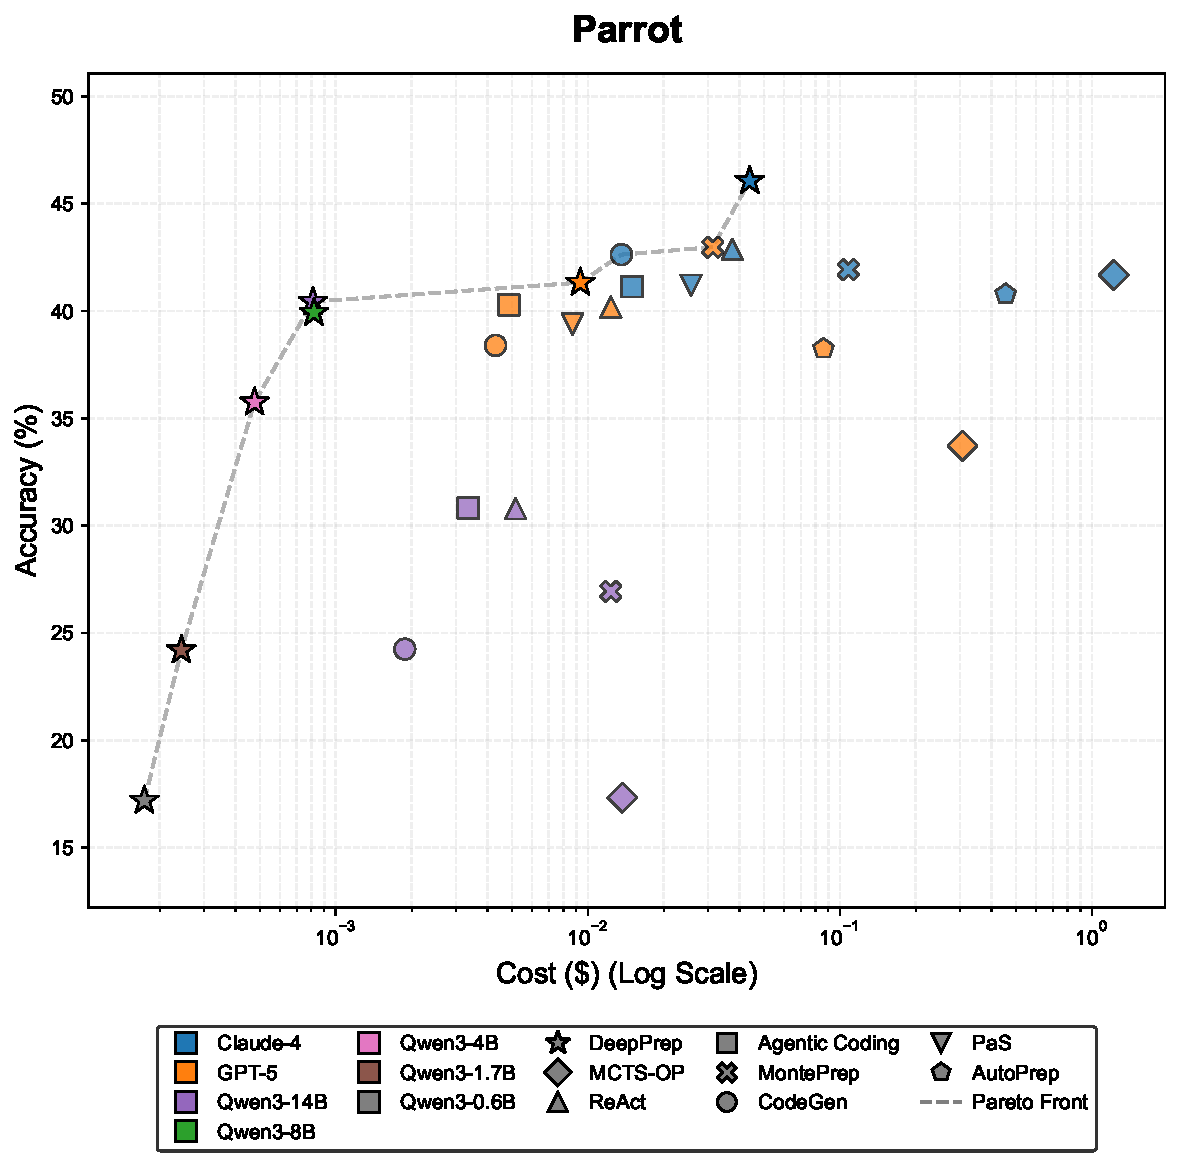
\includegraphics[width=0.99\columnwidth]{plots/plot/pareto_front_parrot.pdf}
    \vspace{-1em} 
    \caption{Pareto Front on Parrot.}
    \label{fig:pareto_front_parrot}
    % \vspace{-1em}
\end{figure}
%!TEX root = ../../main.tex
\begin{figure*}[t]
    \centering 
    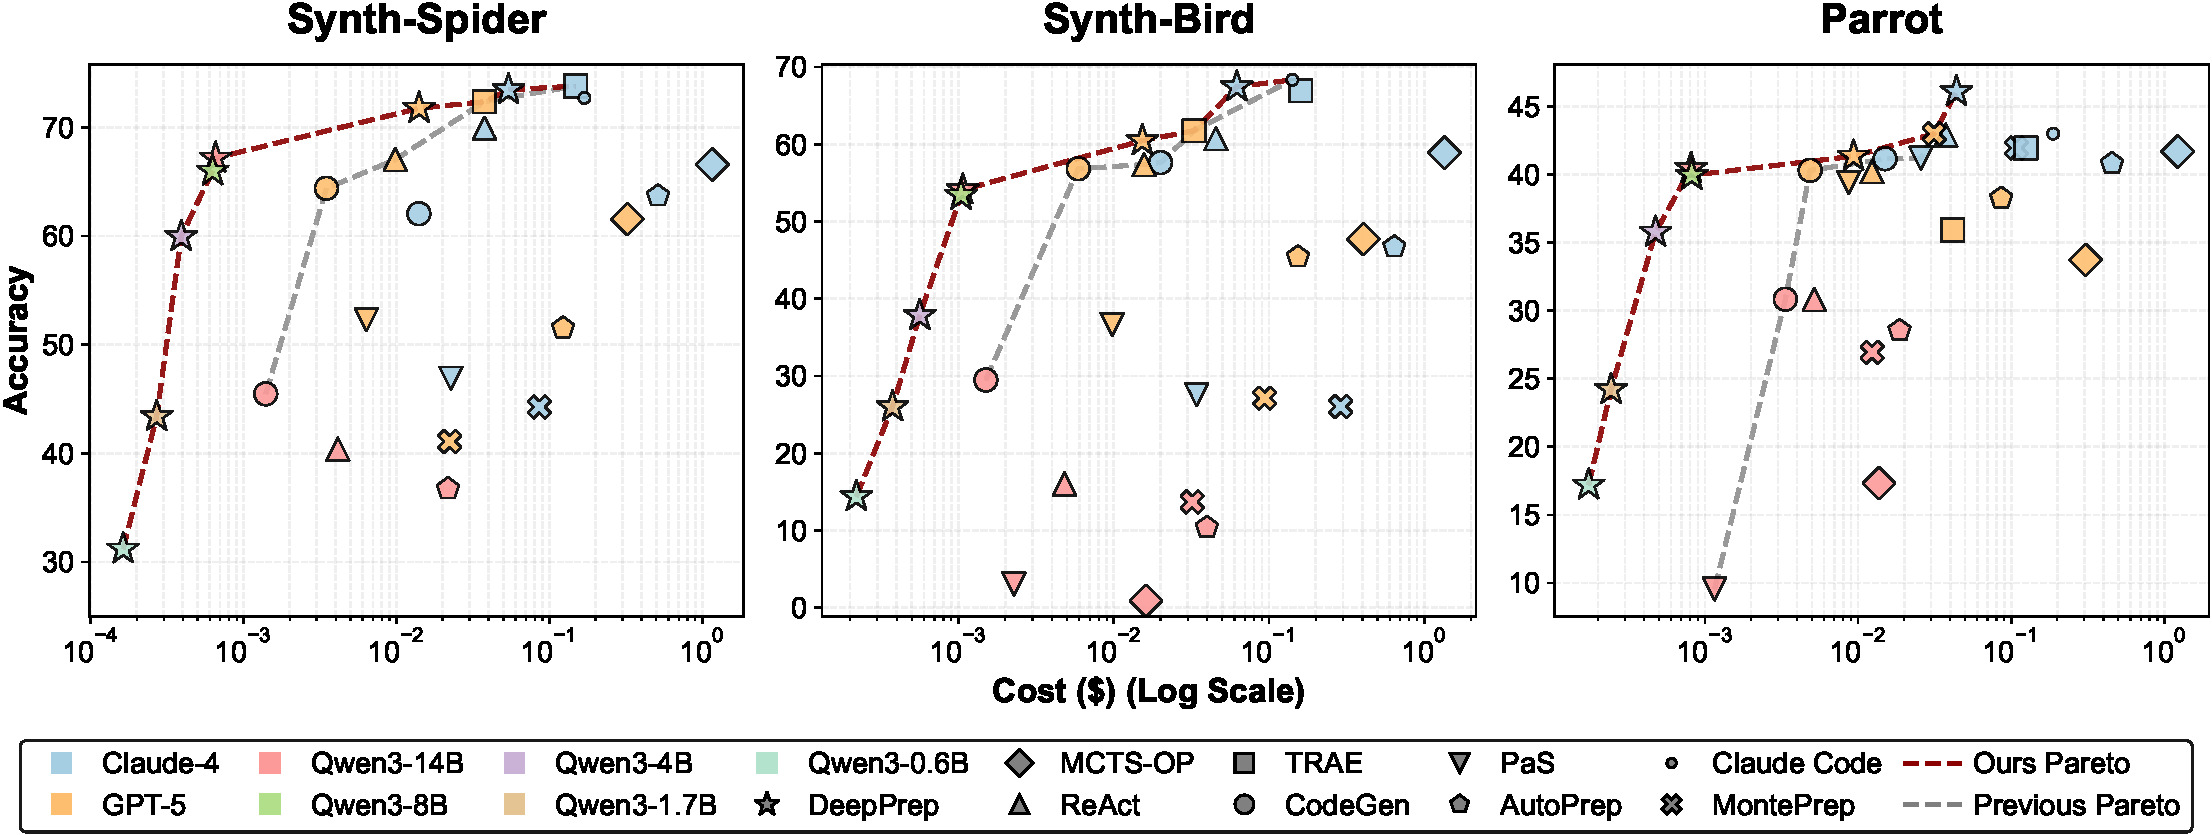
\includegraphics[width=0.7\textwidth]{plots/plot/combined_pareto_front_compare.pdf}
  \vspace{-0.7em}
    \caption{Cost–Accuracy trade-off comparison. Colors represent different LLM backbones, and shapes denote different methods. The red and grey dashed lines indicate the Pareto frontiers of our method and previous baselines, respectively.
    }
    \label{fig:combined_pareto_front_compare}
  \vspace{-1em}
\end{figure*}  



\stitle{Exp-\expnum\label{exp:training_comparison}: Accuracy and Completion Rate Comparison.}
We compare \sys with prompting baselines and training baselines on accuracy and completion rate. 
Results on Qwen3-14B and Qwen3-8B are reported in Table~\ref{tbl:opensource_exp}, as they are strong open-source backbones at two model scales commonly used in code and data tasks. Additional backbone results are presented in later experiments.

\etitle{(1) In-Domain Test.}
\sys achieves the highest accuracy and completion rate across both backbones on the Synth-Spider test set. On Qwen3-14B, it reaches 67.18 accuracy (Table~\ref{subtbl:open_qwen14b}), exceeding the strongest prompting baseline CodeGen by 21.71 points and the strongest training baseline by 5.48 points, with similar gains in completion rate.
% In contrast, the general-purpose data agent DeepAnalyze achieves 35.66 accuracy on the same dataset. 
These gains stem from combining tree-structured exploration with execution-grounded actions, enabling the agent to revise earlier decisions and avoid invalid operator sequences.
% during pipeline construction.

\etitle{(2) Out-of-Domain Test.}
Under the single-source training method, \sys maintains a clear advantage on out-of-domain datasets. On Synth-Bird, \sys (Qwen3-14B) achieves 54.09 accuracy compared with 48.01 for IL, and the 8B model achieves 53.39 versus 43.30. On Parrot, we observe a similar ordering among methods. DeepAnalyze shows much lower performance on Synth-Bird (1.74 accuracy), indicating limited robustness when pipeline length and operator dependencies increase. These results align with our training design, where progressive curriculum and hybrid rewards expose the model to multi-step, feedback-driven reasoning trajectories rather than single-pass program generation.

%\noindent
%\textbf{Exp-\expnum\label{exp:training_comparison}: Accuracy and Complete Rate Comparison.}
%We evaluate the effectiveness of our training strategies by comparing \sys with extensive prompting baselines and training baselines. The results on Qwen3-14B and Qwen3-8B are presented in Table~\ref{tbl:opensource_exp}.

%First, \sys establishes new SOTA results. As shown in Table~\ref{subtbl:open_qwen14b}, \sys (Qwen3-14B) achieves an accuracy of \textbf{67.18} on DP-Spider. This significantly outperforms the best prompting baseline CodeGen by a margin of 21.71 and the best training baselines by a margin of 5.48. Similarly, this advantage is consistent on Complete Rate.
%This substantial improvement validates that the integration of online tree-based agentic reasoning with offline progressive agentic training empowers the agent to autonomously rectify intermediate execution errors and robustly converge to the target schema.
%
%Second, \sys exhibits robust generalization capabilities under the \textit{single-source training, multi-target evaluation} setting. On the complex cross-domain dataset DP-Bird, \sys consistently widens the performance gap against SFT on both backbones. Specifically, \sys (Qwen3-14B) achieves 54.09 accuracy, outperforming SFT (48.01) by a margin of 6.08 points. Similarly, the 8B model achieves 53.39 accuracy, maintaining a strong lead over its SFT baseline (43.30). This indicates that \sys learns the intrinsic reasoning logic of DP rather than merely memorizing schema-specific patterns from the training set. 

%Third, \sys significantly outperforms general-purpose data agents. We observe that DeepAnalyze (Table~\ref{subtbl:open_qwen8b}) struggles in data preparation. While it achieves moderate performance on DP-Spider (35.66), its accuracy collapses to 1.74 on DP-Bird. This highlights the necessity of a dedicated agent for ADP task.
% General agents lack the specialized domain knowledge required to handle multi-hop table transformations. In contrast, \sys leverages high-quality synthesized trajectories to master these domain-specific challenges.

\begin{shaded}
\noindent \textbf{Finding \findingnum: \sys achieves the highest accuracy and completion rate among the compared methods and shows good generalization across datasets.}
\end{shaded}

% \stitle{Finding \findingnum:} \sys achieves the highest accuracy and completion rate among the compared methods and shows good generalization across datasets.

\noindent
\textbf{Exp-\expnum\label{exp:prompting_comparison}: Cost–Accuracy Trade-off Comparison.}
We compare methods under a cost–accuracy trade-off by jointly evaluating accuracy and cost. Figure~\ref{fig:combined_pareto_front_compare} plots prompting baselines and \sys variants across different LLM backbones, and shows two Pareto frontiers: \textit{Previous Pareto}, computed from baselines only, and \textit{Ours Pareto}, computed after adding \sys.

%We further assess \sys's practical utility by jointly considering Exact Matching Accuracy and Inference Cost. Figure~\ref{fig:combined_pareto_front_compare} shows all prompting baselines and \sys variants across different LLM backbones, and overlays two Pareto frontiers: \textit{Previous Pareto}, computed from baselines only, and \textit{Ours Pareto}, computed after adding \sys.

First, \sys lies on or near the Pareto frontier in most settings and extends the frontier across all three datasets. In Figure~\ref{fig:combined_pareto_front_compare}, the \textit{Ours Pareto} curve is shifted toward the upper-left relative to the \textit{Previous Pareto}, meaning that \sys achieves higher accuracy at the same cost, or similar accuracy at lower cost. This appears on Synth-Spider, Synth-Bird, and Parrot, indicating that the cost–accuracy advantage is consistent across datasets and backbones.

Second, \sys reaches accuracy close to strong closed-source baselines at substantially lower cost. On Synth-Spider, \sys (Qwen3-14B) achieves 67.18 accuracy at a very low cost, achieving a comparable accuracy with ReAct on Claude-4 (69.92 accuracy) while reducing cost by about 57$\times$. 
This is attributed to our design that uses structured tree-based reasoning to guide smaller or open models toward valid pipelines with fewer failed executions.

\revise{Third, compared with the agentic coding systems TRAE and Claude Code, \sys achieves comparable accuracy at much lower cost. 
For example, with GPT-5, \sys achieves accuracy comparable to TRAE while reducing cost by 2.7$\times$ on Synth-Spider. This further demonstrates the cost-effectiveness of \sys.}

%Third, \sys remains competitive under more complex scenarios. On Synth-Bird, several search-based baselines show noticeably lower accuracy (\eg MontePrep around 25), whereas \sys continues to appear on the Pareto frontier. A similar trend is observed on Parrot. This suggests that the cost–accuracy behavior of \sys is stable when pipeline length increases.


\begin{shaded}
\noindent \textbf{Finding \findingnum: \sys extends the cost–accuracy Pareto frontier, achieving accuracy close to strong closed-source baselines at substantially lower inference cost.}
\end{shaded}
\subsection{Ablation Studies}
\label{expsec: ablation_on_policy_learning}

\revise{

\begin{table}[t]
    \centering
    \caption{\bf Overall Ablation Study on Qwen3-8B. PAT represents Progressive Agentic Training and TAR represents Tree-based Agentic Reasoning.}
    \vspace{-1em}
    \label{\labelprefix tbl:overall_ablation_study}
    \resizebox{0.9\linewidth}{!}{
    \begin{tabular}{|c||c|c|c|c|c|c|}
        \hline
        \multirow{2}{*}{\textbf{Method}} 
        & \multicolumn{2}{c|}{\textbf{Synth-Spider}} 
        & \multicolumn{2}{c|}{\textbf{Synth-Bird}} 
        & \multicolumn{2}{c|}{\textbf{Parrot}} \\ 
        \cline{2-7}
        & \textbf{Acc.} & \textbf{Comp.} 
        & \textbf{Acc.} & \textbf{Comp.} 
        & \textbf{Acc.} & \textbf{Comp.} \\
        \hline \hline
        DeepPrep 
        & \textbf{65.99} & \textbf{97.46\%} 
        & \textbf{53.39} & \textbf{92.78\%} 
        & \textbf{39.93} & \textbf{98.46\%} \\
        
        w/o PAT
        & 22.21 & 59.76\% 
        & 8.87 & 41.90\% 
        & 25.27 & 70.62\% \\
        
        w/o PAT, TAR
        & 4.68 & 7.42\% 
        & 0.65 & 4.33\% 
        & 3.09 & 8.32\% \\
        \hline
    \end{tabular}
    }
    \vspace{-1.5em}
\end{table}


\stitle{Exp-\expnum\label{exp:ablation_analysis_overall}: Overall Ablation Studies of \sys.} We evaluate the contribution of two modules (TAR and PAT) in \sys. The results are reported in Table~\ref{\labelprefix tbl:overall_ablation_study}.
% The results show that the performance gains cannot be explained solely by stronger backbone models. 
As reported, removing PAT while retaining TAR causes substantial degradation, reducing accuracy by 43.78 on Synth-Spider, 44.52 on Synth-Bird, and 14.66 on Parrot. This indicates that the model must first learn the operator syntax and reasoning protocol before tree-based reasoning can be effectively utilized.
Further removing TAR causes the method to degenerate into single-turn operator generation, leading to a larger performance drop (by 61.31 on Synth-Spider). Meanwhile, the completion rate falls to near-zero levels. This demonstrates that TAR is critical for leveraging execution feedback, and recovering from erroneous decisions through backtracking.
}

\begin{table}[t]
    \centering
    \caption{\bf Detailed Ablation Studies on PAT (Qwen3-8B).}
    \vspace{-1em}
    \label{tbl:ablation_results_split}
    
    % --- Subtable 1: Cold Start ---
    \begin{subtable}[t]{0.88\columnwidth}
        \centering
        \caption{\bf{Ablation study on Cold Start stage. OSL represent Operator syntax Learning module in Section~\ref{subsec:cold_start}.}}
        \label{subtbl:cold_start}
        \vspace{-0.5em}
        \resizebox{0.99\linewidth}{!}{
        \begin{tabular}{|c||c|c|c|c|c|c|}
            \hline
            \multirow{2}{*}{\textbf{Method}} & \multicolumn{2}{c|}{\textbf{Synth-Spider}} & \multicolumn{2}{c|}{\textbf{Synth-Bird}} & \multicolumn{2}{c|}{\textbf{Parrot}} \\ \cline{2-7}
             & \textbf{Acc.} & \textbf{Comp.} & \textbf{Acc.} & \textbf{Comp.} & \textbf{Acc.} & \textbf{Comp.} \\
            \hline \hline
            % Row 1: Curriculum SFT
            Cold-Start & \textbf{60.66} & \textbf{91.63\%} & \textbf{45.27} & \textbf{81.39\%} & \textbf{36.22} & \textbf{92.16\%} \\
            % Row 2: w/o Operator Learning
            w/o OSL & {59.65} & {90.54\%} & {43.30} & {80.43\%} & {36.15} & {91.08\%} \\
            \hline
        \end{tabular}
        }
    \end{subtable}
    
    \vspace{0.5em}
    
    % --- Subtable 2: Multiturn RL ---
    \begin{subtable}[t]{0.93\columnwidth}
        \centering
        \caption{\bf{Ablation study on the reward of Multiturn RL stage.}}
        \label{subtbl:rl_stage}
        \vspace{-0.5em}
        \resizebox{0.99\linewidth}{!}{
        \begin{tabular}{|c||c|c|c|c|c|c|}
            \hline
            \multirow{2}{*}{\textbf{Method}} & \multicolumn{2}{c|}{\textbf{Synth-Spider}} & \multicolumn{2}{c|}{\textbf{Synth-Bird}} & \multicolumn{2}{c|}{\textbf{Parrot}} \\ \cline{2-7}
             & \textbf{Acc.} & \textbf{Comp.} & \textbf{Acc.} & \textbf{Comp.} & \textbf{Acc.} & \textbf{Comp.} \\
            \hline \hline
            % Row 1: V0-v1-v2 (Full sysem)
            \sys & \textbf{65.99} & \underline{97.46\%} & \textbf{53.39} & \underline{92.78\%} & \textbf{39.93} & \underline{98.46\%} \\
            % Row 2: v0-v1 (w/o R_llm)
            w/o $R_{\text{llm}}$ & \underline{64.54} & 96.96\% & \underline{51.67} & 92.31\% & \underline{39.12} & 94.21\% \\
            % Row 3: v0 (w/o R_llm, R_part)
            w/o $R_{\text{llm}}, R_{\text{part}}$ & 61.85 & \textbf{98.71\%} & 47.15 & \textbf{95.57\%} & 37.22 & \textbf{99.34\%} \\
            \hline
        \end{tabular}
        }
    \end{subtable}
    
  \vspace{-1em}
\end{table}


\stitle{Exp-\expnum\label{exp:ablation_analysis}: Detailed Ablation Studies on Progressive Agentic Training.}
We evaluate the contribution of specific components within our progressive agentic training. The results are detailed in Table~\ref{tbl:ablation_results_split}. 

Table~\ref{subtbl:cold_start} demonstrates that cold-start curriculum is useful. Removing this component causes a simultaneous decline in both accuracy and completion rate across all datasets. For instance, the completion rate on Synth-Spider drops from 91.63 to 90.54.
Because this component familiarizes the model with the operator syntax and parameters. Without it, the model tends to generate non-executable actions and fail to complete the reasoning trajectory. 

Table~\ref{subtbl:rl_stage} validates the design of our reward function in RL.
First, removing process reward ($R_{\text{llm}}$) results in an accuracy drop, which shows that $R_{\text{llm}}$ prevents ``reward hacking''. Without semantic verification, the policy learns to satisfy superficial schema constraints, such as renaming columns, while neglecting the actual data transformation logic.
Second, relying solely on outcome rewards (w/o $R_{\text{out}}, R_{\text{part}}$) yields the highest completion rate but the lowest accuracy.
This suggests that sparse rewards induce conservative behavior. The agent avoids complex exploration or backtracking to minimize the risk of runtime errors. Thus, it prioritizes safe but incorrect paths to ensure the episode terminates successfully.

\begin{shaded}
\noindent \textbf{Finding \findingnum \&\findingnum: Each key component of \sys contributes to its overall performance.
}
\end{shaded}
% \revise{\subsection{Effectiveness of Training Data Synthesis}
\label{subsec:data_effectiveness}

% \begin{figure}[t]
    \centering
    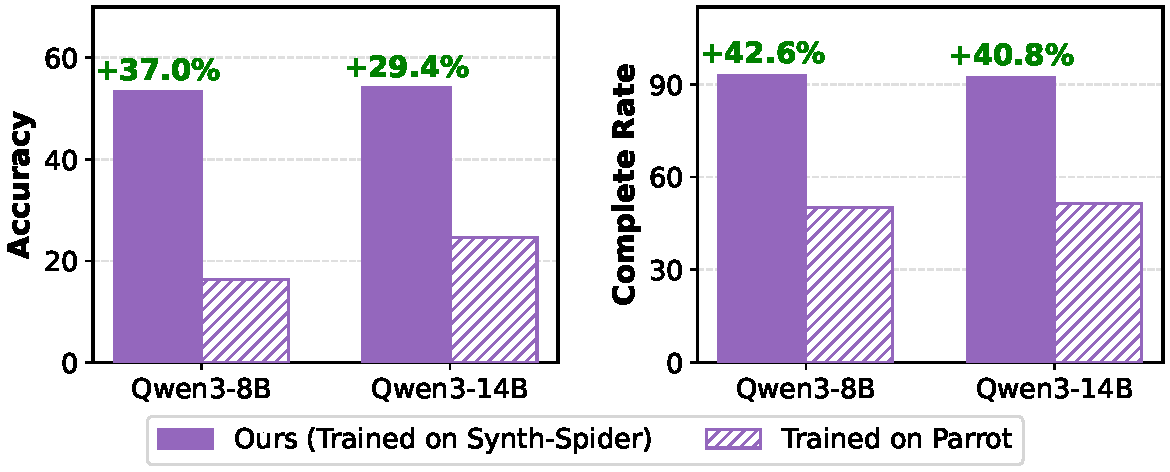
\includegraphics[width=0.99\columnwidth]{plots/plot/trained_on_spider_and_parrot_eval_bird.pdf}
    \vspace{-0.5em} 
    \caption{Evaluation results on Synth-Bird (Dev) of models trained on Synth-Spider (Train) and Parrot (Train).}
    \label{fig:trained_on_spider_and_parrot_eval_bird}
    \vspace{-0.5em}
\end{figure}
% \begin{figure}[t]
    \centering
    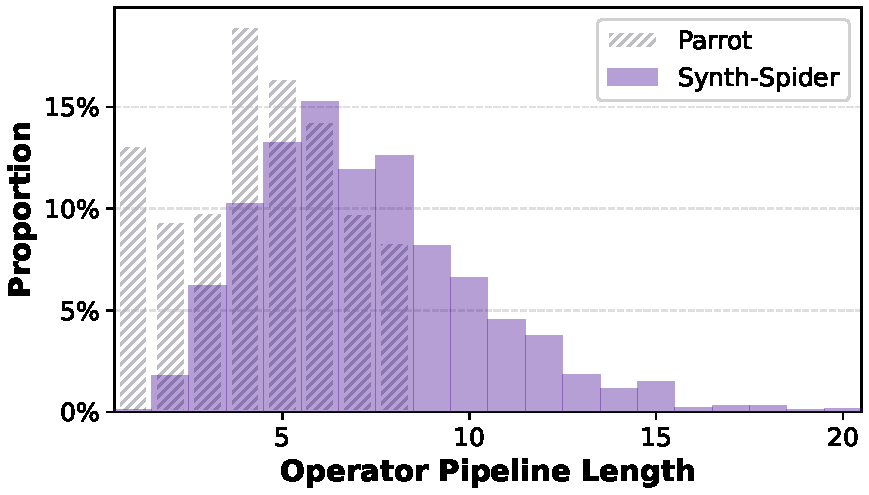
\includegraphics[width=0.95\columnwidth]{plots/plot/op_len_distribution.pdf}
    \vspace{-1em} 
    \caption{Operator Pipeline Length Distribution.}
    \label{fig:op_len_distribution}
    \vspace{-0.5em}
    % \vspace{-1em}
\end{figure}
\begin{figure}[t]
    \centering
    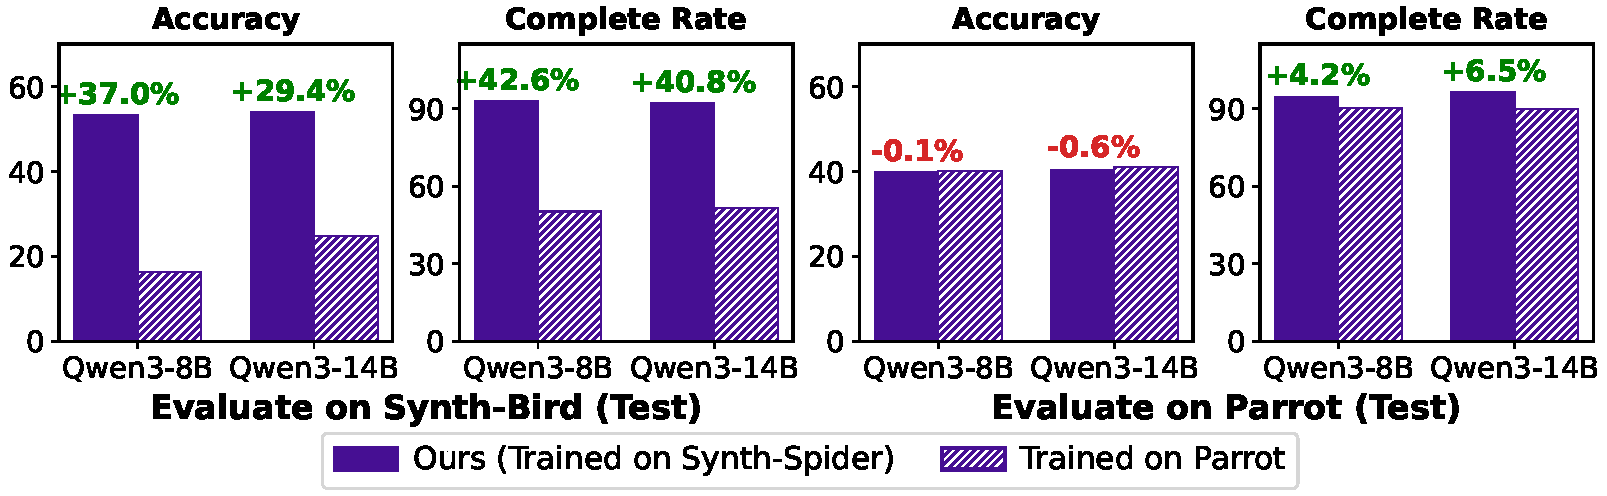
\includegraphics[width=1.01\columnwidth]{plots/plot/trained_on_spider_and_parrot.pdf}
    \vspace{-2em} 
    \caption{Evaluation results of models trained on Synth-Spider (Train) and Parrot (Train).}
    \label{\labelprefix fig:trained_on_spider_and_parrot}
    \vspace{-1em}
\end{figure}

\stitle{Exp-\expnum\label{exp:data_effectiveness}: Effectiveness of Synthesized Training Data.}
We evaluate whether models trained on our synthesized Synth-Spider training set generalize better than those trained on the public Parrot training set. 
% Both models are evaluated on the Synth-Bird Test set.
We first evaluate these two models on Synth-Bird (Test) under the out-of-domain setting. As illustrated on the left part of Figure~\ref{fig:trained_on_spider_and_parrot}, training on Synth-Spider yields much higher performance: accuracy increases by 37.0 and 29.4 points on Qwen3-8B and Qwen3-14B over Parrot. 
% Completion rate shows even larger gains, with increases of 42.6 and 40.8 respectively.
To further highlight the effectiveness of synthesized data, we adopt a more challenging setting. We evaluate on Parrot (Test) of models trained on Synth-Spider (totally out-of-domain setting) and models trained on Parrot (in-domain setting). As illustrated on the right of Figure~\ref{fig:trained_on_spider_and_parrot}. Our synthesized data is even competitive under such challenging experiment setting. Models trained on Synth-Spider achieve comparable accuracy to the model trained on Parrot (40.44 vs. 40.99 on Qwen3-8B). 

% These consistent gains show that our synthesized training data provide more effective supervision for agentic training than existing public data.
% The stronger generalization of Synth-Spider lies in the diversity and complexity of synthesized DP pipelines.
% First, as shown in Table~\ref{tbl:datasets}, Synth-Spider has more long-horizon operator and provides broader operator coverage than Parrot. Second, Synth-Spider has more diverse operator combination. We have conducted a fine-grained analysis of operator compositional diversity between these two datasets. Synth-Spider produces 496 unique bigrams and 2,875 unique trigrams, compared to Parrot’s 189 and 758 respectively. Moreover, Synth-Spider’s top-5 and top-10 bigram concentration ratios are also lower than Parrot’s (0.226 and 0.326 vs. 0.248 and 0.361), indicating that its operator distribution is less dominated by a few frequent patterns.
% In summary, the more diverse and complex pipelines in Synth-Spider promotes tree-based agentic reasoning during agentic training, in turn improving generalization capabilities to unseen data.


% To understand why Synth-Spider yields stronger generalization, we compare operator-pipeline length distributions of the two training datasets in Figure~\ref{fig:op_len_distribution}. Parrot samples cluster on shorter pipelines, while Synth-Spider consistently contains more medium- and long-horizon operator pipelines.
% This adds procedural complexity to promotes tree-based agentic reasoning during agentic training, in turn improving generalization capabilities to unseen data.

\begin{shaded}
\noindent \textbf{Finding \findingnum: 
Our synthetic training data provides effective supervision for agentic training, significantly improving the performance on unseen tasks.
%Our data synthesis strategy fosters robust planning, significantly improving task completion rates on unseen tasks without compromising accuracy.
}
\end{shaded}}
% \subsection{Model Scaling Study}
\label{subsec:scalability}

\begin{figure}[t]
    \centering
    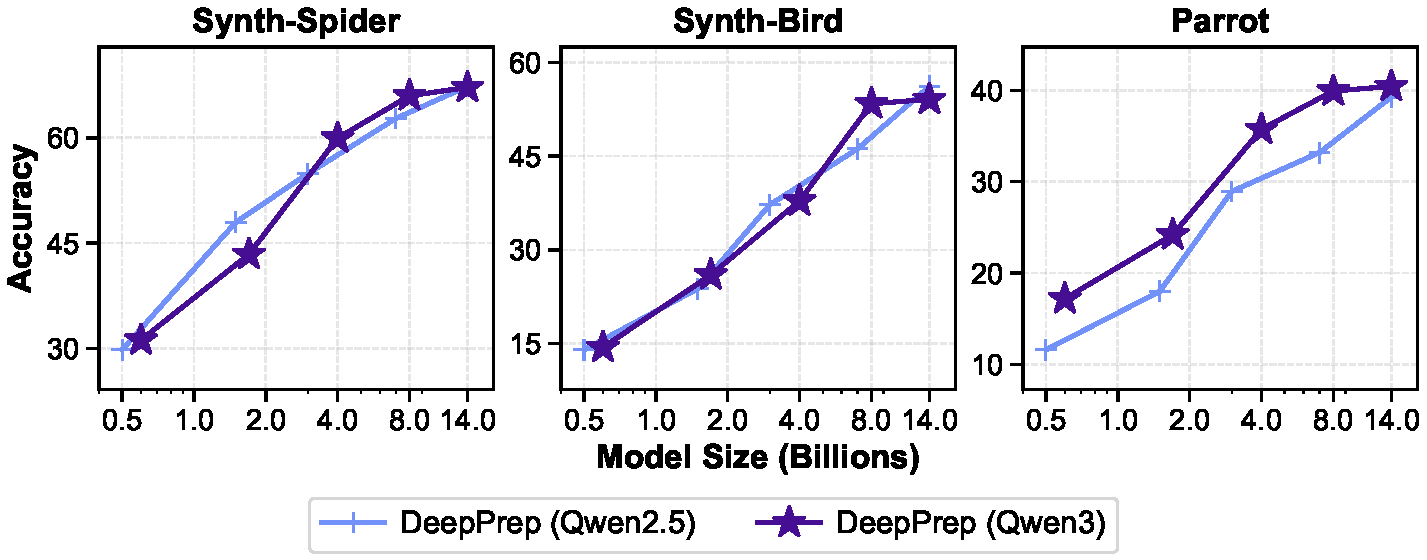
\includegraphics[width=1.01\columnwidth]{plots/plot/performance_scale_accuracy_only.pdf}
    \vspace{-1.5em} 
    \caption{Performance scales with larger model size.
    % \fmh{Results of Qwen2.5 are not updated (Use 2025 version).} 
    }
    \label{\labelprefix fig:performance_scale_accuracy_only}
    \vspace{-0.5em} 
  %\vspace{-1em}
\end{figure}

\stitle{Exp-\expnum\label{exp:model_scaling}: Model Scaling Study.}
We study how \sys performs under different backbone model sizes. We train \sys with LLM backbones ranging from 0.5B to 14B parameters across the Qwen2.5 and Qwen3 families.
Figure~\ref{\labelprefix fig:performance_scale_accuracy_only} shows that accuracy steadily increases with model size. On Synth-Spider, scaling Qwen3 from 0.6B to 14B improves Accuracy from 31.20 to 67.18. Across comparable model sizes, the Qwen3 series also shows stronger out-of-domain performance than Qwen2.5. For example, on Synth-Bird, Qwen3-8B achieves 53.39 Accuracy versus 46.17 for Qwen2.5-7B. These results suggest \sys benefits from stronger backbone models and maintains positive scaling trends.

%\noindent
%\textbf{Exp-\expnum\label{exp:scalability}: Can the performance of \sys scale with increasing model sizes?}
%To answer this, we trained \sys using different LLM backbones (Qwen2.5 and Qwen3) ranging from 0.5B to 14B parameters, totaling 10 models. As shown in Figure~\ref{\labelprefix fig:performance_scale_accuracy_only}, Accuracy improves consistently as the model size increases. Specifically, on Synth-Spider, scaling Qwen3 from 0.6B to 14B boosts Accuracy from 31.20 to 67.18. Furthermore, we find that Qwen3 series shows stronger generalization capability than Qwen2.5 series. For example, on the complex Synth-Bird dataset, Qwen3-8B achieves 53.39 accuracy, outperforming Qwen2.5-7B (46.17). The experimental results indicate that 
%\sys can improve further as stronger open-source models are released.

\begin{shaded}
\noindent
\textbf{Finding \findingnum: The performance of \sys improves with larger backbone model sizes, which suggest that \sys benefits from stronger backbone models and maintains positive scaling trends.}
\end{shaded}
\subsection{In-Depth Analysis}
\label{subsec:in_depth_analysis}

\begin{figure}[t]
    \centering
    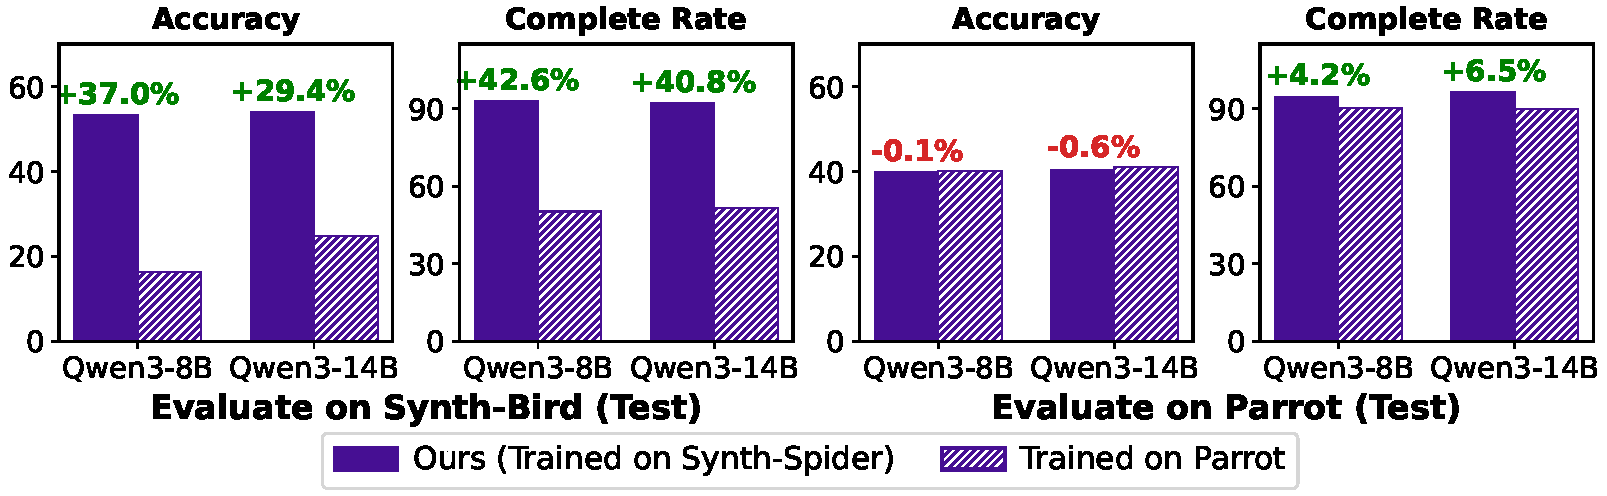
\includegraphics[width=1.01\columnwidth]{plots/plot/trained_on_spider_and_parrot.pdf}
    \vspace{-2em} 
    \caption{Evaluation results of models trained on Synth-Spider (Train) and Parrot (Train).}
    \label{\labelprefix fig:trained_on_spider_and_parrot}
    \vspace{-1em}
\end{figure}
\revise{

\stitle{Exp-\expnum\label{exp:data_effectiveness}: Effectiveness of Synthesized Training Data.}
We evaluate whether models trained on our synthesized Synth-Spider dataset generalize better than those trained on the public Parrot dataset. 
% Both models are evaluated on the Synth-Bird Test set.
We first evaluate these two models on Synth-Bird (Test) under the out-of-domain setting. As illustrated in the left of Figure~\ref{fig:trained_on_spider_and_parrot}, training on Synth-Spider yields much higher performance: accuracy increases by 37.0 and 29.4 points on Qwen3-8B and Qwen3-14B over Parrot. 
% Completion rate shows even larger gains, with increases of 42.6 and 40.8 respectively.
To further highlight the effectiveness of synthesized data, we adopt a more challenging setting. We evaluate models trained on Synth-Spider under a totally out-of-domain setting and models trained on Parrot under an in-domain setting on Parrot (Test), as illustrated in the right of Figure~\ref{fig:trained_on_spider_and_parrot}. Our synthesized data are still competitive under such a challenging experimental setting. Models trained on Synth-Spider achieve accuracy comparable to models trained on Parrot (40.44 vs. 40.99 on Qwen3-8B).

\begin{shaded}
\noindent \textbf{Finding \findingnum: 
Our synthetic training data provides effective supervision for agentic training, significantly improving the performance on unseen tasks.
}
\end{shaded}
}



\revise{
\begin{table}[t]
  \centering
  \caption{\bf Results on the Buildings dataset (real-world).}
  \vspace{-1em}
  \label{\labelprefix tbl:buildings_exp}
  \resizebox{0.68\columnwidth}{!}{
    \begin{tabular}{|c||c|c|c|}
      \hline
      \textbf{Method} & \textbf{Acc.} & \textbf{Comp.} & \textbf{Cost (\$)} \\
      \hline \hline
      % CodeGen & 71.43 & 95.24\% & \textbf{0.0017} \\
      ReAct & 74.29 & 99.05\% & \textbf{0.0052} \\
      CodeGen & 71.43 & 100\% & 0.0054 \\
      MontePrep & 72.38 & 86.67\% & 0.043 \\
      MCTS-OP & 69.52 & 99.05\% & 0.057 \\
      \hline \hline
      \textbf{\sys (Ours)} & \textbf{82.85} & \textbf{100\%} & {0.0082} \\
      \hline
    \end{tabular}
  }
  \vspace{-1em}
\end{table}


\stitle{Exp-\expnum\label{exp:building_exp}: Generalization on Real-World Dataset.}
We have compared \sys with prompting baselines on the real-world dataset Buildings~\cite{sharma2023automatic}. Table~\ref{\labelprefix tbl:buildings_exp} reports Accuracy, Completion Rate and API Cost per case. As illustrated, \sys generalizes well on the real-world dataset. Specifically, \sys achieves the best Accuracy of 82.85 and maintains relatively low inference
cost (0.008\$ per case). This enhances its usability in real-world.

\stitle{Error Analysis.} We further conduct an error analysis of this experiment and identify two key challenges in real-world scenarios. (1) Real cases often contain abbreviated or domain-specific column names, leading to selecting the wrong columns required to be mapped into the target columns. (2) The target specification in real cases is often under-specified. For example, whether daily or monthly granularity is expected is not specified clearly in the requirement. We will address these challenges in our future work. The complete statistics can be found in our technical report~\cite{technical_report}.

\begin{shaded}
\noindent
\textbf{Finding \findingnum: \sys generalizes well to the real-world Buildings dataset.}
\end{shaded}}

\revise{

\begin{figure}[t]
    \centering
    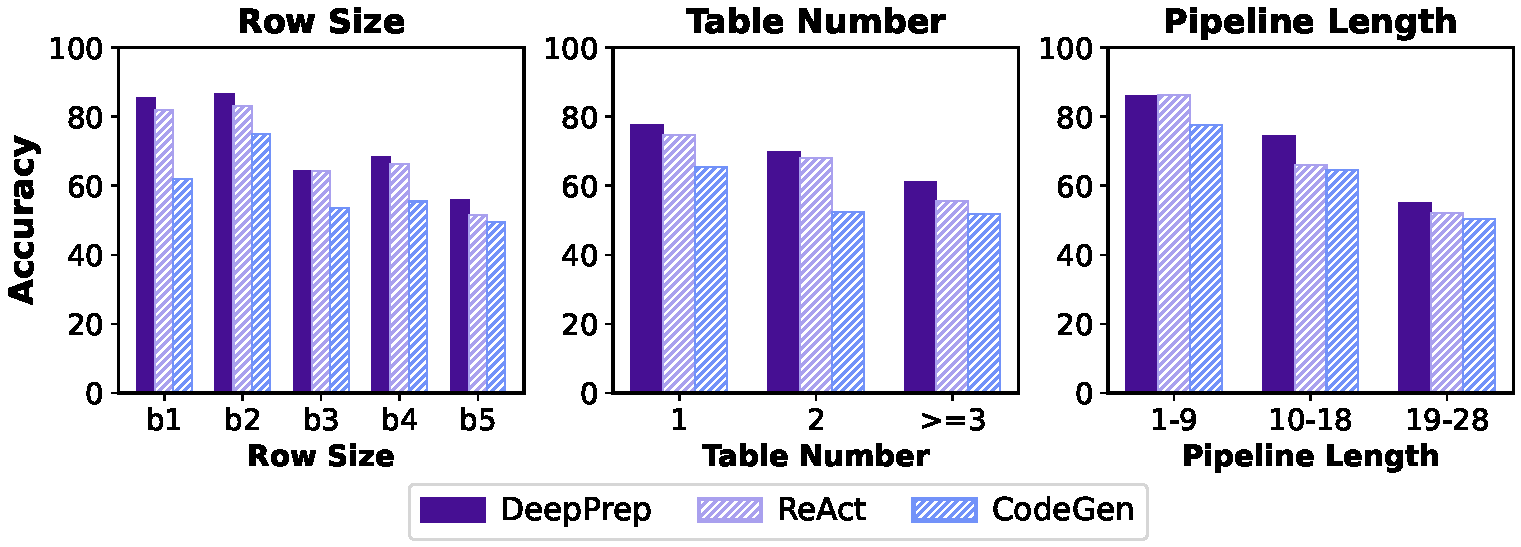
\includegraphics[width=0.99\columnwidth]{figures/fig/overview_synth_spider.pdf}
    \vspace{-1em}
    \caption{Scalability analysis on Synth-Spider with varying (a) row size, (b) source table number, and (c) pipeline length.}
    \label{fig:scalability_synth_spider}
    \vspace{-1em}
\end{figure}


\stitle{Exp-\expnum\label{exp:scalability}: Scalability Analysis.}
We evaluate the scalability of \sys on Synth-Spider from three dimensions: row size, number of source tables, and pipeline length.
% and report the accuracy results, time usage and resource usage. 

\stitle{Scalability Analysis of Accuracy.} As shown in Figure~\ref{fig:scalability_synth_spider}(a), \sys remains robust on small and medium-sized tables. Performance degrades only for the largest row-size bucket ($b_5$: 36 to 124k+ rows), where accuracy decreases by 29.54 points compared with the smallest bucket ($b_1$: 1 to 9 rows). This degradation is primarily caused by the table sampling strategy used to control token usage, where relevant information may be omitted from the sampled content. As shown in Figure~\ref{fig:scalability_synth_spider}, performance decreases as more source tables are involved, but \sys consistently achieves the highest accuracy across different table number groups. As illustrated, all methods degrade as the pipeline length increases.
% , reflecting the greater difficulty of long-horizon pipeline construction. 
However, \sys shows the smallest degradation, and its advantage over baselines becomes larger on complex cases. 

\stitle{Scalability Analysis of Time and Resource Usage.} \sys exhibits stable growth in both execution time and memory usage as workload complexity increases. For example, on Synth-Spider, the average execution time increases only from 8.91 to 11.30 seconds when moving from the smallest to the largest column-size bucket, while memory usage remains between 66 MB and 69 MB. The stable scaling behavior can be explained by the generative search framework, as defined in Section~\ref{sec:tree_based_agentic_reasoning}. The process is bounded by the maximum exploration turn $T$ and the maximum operator sequence length $L$ per expansion, yielding a worst-case complexity of $O(T\times L)$. Unlike MCTS-based methods, \sys generates only one operator pipeline conditioned on the current tree state. The ``pruning'' is implicit in the LLM’s decision-making. Consequently, the effective branching factor depends on the LLM’s learned policy and remains bounded regardless of input size, which explains the stable growth in time and memory usage.

Complete scalability results across all datasets and detailed time and resource usage analysis are provided in our technical report~\cite{technical_report}.

\begin{shaded}
\noindent
\textbf{Finding \findingnum: \sys maintains robust accuracy and stable resource usage as workload complexity increases.}
\end{shaded}

}



